\documentclass[a4paper,12pt]{report}
%%%%%%%%%%%%%%%%%%%%%%%%%%%%%%%%%%%%%%%%%%%%%%%%%%%%%%%%%%%%%%%%%%%%%%%%%
%%%%%% Definizioni:
\def\titolotesi{Smart City dalla teoria alla pratica} % INSERIRE TIOLO DELLA TESI
\def\laureando{Pietro Palazzo}       % INSERTIRE NOME COGNOME LAUREANDO
\def\annoaccademico{2017--2018}    % INSERIRE ANNO ACCADEMICO
\def\dedica{Dedica...}      % INSERIRE DEDICA

% Title Page
\title{\begin{large}\textbf{\titolotesi}\end{large}}
\author{\laureando}
\usepackage[italian]{babel}
\usepackage[T1]{fontenc}
\usepackage[utf8x]{inputenc}
\usepackage{minted}
\usepackage[square,numbers]{natbib}
\usepackage{listings}
\usepackage{color}
\usepackage[colorlinks=true]{hyperref}
\hypersetup{
	bookmarksnumbered=true,
	linkcolor=black,
	citecolor=black,
	pagecolor=black,
	urlcolor=black,
}
\definecolor{lightgray}{rgb}{.9,.9,.9}
\definecolor{darkgray}{rgb}{.4,.4,.4}
\definecolor{purple}{rgb}{0.65, 0.12, 0.82}

\lstdefinelanguage{JavaScript}{
  keywords={typeof, new, true, false, catch, function, return, null, catch, switch, var, if, in, while, do, else, case, break, Number},
  keywordstyle=\color{blue}\bfseries,
  ndkeywords={class, export, boolean, throw, implements, import, this},
  ndkeywordstyle=\color{darkgray}\bfseries,
  identifierstyle=\color{black},
  sensitive=false,
  comment=[l]{//},
  morecomment=[s]{/*}{*/},
  commentstyle=\color{purple}\ttfamily,
  stringstyle=\color{red}\ttfamily,
  morestring=[b]',
  morestring=[b]"
}
\lstset{
   language=JavaScript,
   backgroundcolor=\color{lightgray},
   extendedchars=true,
   basicstyle=\fontsize{9}{13}\selectfont\ttfamily,%\footnotesize\ttfamily,
   showstringspaces=false,
   showspaces=false,
   numbers=left,
   numberstyle=\footnotesize,
   numbersep=9pt,
   tabsize=2,
   breaklines=true,
   showtabs=false,
   captionpos=b,
}
\usepackage{url}

\usepackage{fancyhdr}
\fancyhf{}
\fancyhead[RO]{\the\chaptermark}
\fancyfoot[LE,RO]{ \thepage \hfil}
\usepackage{epsfig}
\pagenumbering{roman}
%\usepackage{setspace}
\newlength\sinistra
\newlength\corpo
\newlength\pagina
\setlength {\pagina} {21cm}
\setlength {\sinistra} {1.46cm}
\setlength {\corpo} {13.5cm}
\textwidth \the\corpo
\hoffset \the\sinistra
\paperwidth \the\pagina
\linespread{1.6}

\graphicspath{ {./images/} }

\begin{document}

\begin{titlepage}
 \begin{center}
\textsc{\Large Universit\`a degli Studi di Perugia}\medskip\\

{\Large Dipartimento di Matematica e Informatica}\medskip\\

\rule{10mm}{0.01mm}\medskip\\

{\small \textsc{Corso di Laurea Magistrale in Informatica}}\medskip\\

\vspace*{3mm}


\includegraphics[scale=0.70]{logounipg.png}

\Large Tesi di Laurea \par\bigskip

{\large \bf \titolotesi \par}

\end{center}\par

\hspace{0.05cm}Laureando:\hspace{7.3cm}Relatore:\par

\hspace{0.0cm}\emph{\laureando}\hfill\emph{Prof.~Osvaldo Gervasi}\\

\hspace{10cm}Tutor:\par

\hfill\emph{ecosteer - Daniel Grazioli}\\

\vfill

\begin{center}
\rule{40mm}{0.01mm}\\
Anno Accademico \annoaccademico
\end{center}
\end{titlepage}
\newpage

% DEDICA
\vspace*{\stretch{1}}
\begin{flushright}
\noindent
A mio padre, per aver detto l'essenziale
\end{flushright}
\vspace*{\stretch{6}}
\cleardoublepage

% CITAZIONE
\vspace*{\stretch{1}}
\begin{flushright}
\noindent
Questa nostra terra, che un tempo ci sembrava infinitamente grande, deve essere considerata nella sua piccolezza. Viviamo in un sistema chiuso, dipendenti gli uni dagli altri e dipendenti tutti dalla terra stessa. Tutto ciò che ci divide è infinitamente meno importante del pericolo che ci unisce.

\textit{Charles Darwin}
\end{flushright}
\vspace*{\stretch{6}}
\cleardoublepage

%%%%%%%%%%%%%%%%%%%%%%%%%%%%%%%%%
\tableofcontents
\listoffigures
%%%% fine prologo

%%%% Inizio corpo tesi
\pagestyle{fancy}
\fancyhead[RO]{\bfseries Introduzione}
\addcontentsline{toc}{chapter}{Introduzione}

\chapter*{Introduzione}

\pagenumbering{arabic}

L'Introduzione non viene numerata...

Nel capitolo \ref{cap1} viene mostrata........




%%%%%%%%%%%%%%%%%%%%%%%%%%%%%%%%%%%%%%%%%%%%%%%%%%%%%%%%%%%%%%%%%%%%%%%%%%%%%%%%%%%%%
%%% CHAPTERS

\chapter{Cos'è una Smart City\label{cap1}}
\fancyhead[RO]{\bfseries Cos'è una Smart City}

Secondo le Nazioni Unite (UN) \cite{UNProjection}, entro il 2050, il 68\% della popolazione mondiale, circa 2.5 miliardi di persone, vivrà in città. Pertanto è fondamentale chiedersi in che modo è possibile rendere questa crescita sostenibile per i cittadini, quindi migliorando i trasporti pubblici, la sicurezza e più in generale la qualità della vita, ma anche e sopratutto per l'ambiente, cercando di ridurre le emissioni e migliorando l'efficienza energetica.

Techopedia definisce \cite{SmartCityDefinition} una città intelligente come quella che incorpora le tecnologie per migliorare le funzioni della città e la qualità della vita dei suoi cittadini. La vivibilità è un fattore chiave nelle città intelligenti e quindi parte dei loro principi guida è di ridurre al minimo l'uso delle risorse, evitare sprechi e ridurre i costi complessivi. Più in generale, l'obiettivo delle smart cities è quello di migliorare la qualità della vita dei cittadini attraverso tecnologie moderne.

Negli anni sono nati vari progetti in tutto il mondo con focus vari e vision diverse: focus sul miglioramento della vita dei cittadini, focus sulla sicurezza, sull' efficientamento energetico o dei trasporti; Per Munish Khetrapal, il direttore del programma smart city e Iot in Cisco, già 5000 città sono sul cammino per diventare smart city.
La discussione su quale sia "il cammino" da intraprendere è ancora aperta, secondo lo smart cities council si possono evidenziare 4 step essenziali:
\begin{itemize}
\item Definizione degli obiettivi che si vogliono raggiungere e della vision. 
\item Definire come usare la tecnologia per migliorare vivibilità, lavoro e sostenibilità connettendo parti del governo pubblico, i cittadini e le imprese del territorio.
\item Definizione di KPI
\item Analisi dei dati ricevuti dai sistemi informatici per capire la situazione corrente e predire quale sarà la successiva.
\end{itemize}

\section{Vivere in una smart city}
Mi sveglio alle 7:00, la mia sveglia connessa inonda la camera di una luce leggera per simulare l'alba e una musica dolce mi sveglia gentilmente. Le serrande si aprono automaticamente mostrando una giornata uggiosa ma la temperatura della camera è perfetta grazie al termostato che ha autoregolato la temperatura della casa. Mentre guardo fuori, ricevo una notifica dalla caffettiera, il caffè è pronto e l'odore mi convince ad alzarmi. 
Finita colazione, guardo l'app dei bus autonomi, ne passerà uno tra 10 minuti. Alla fermata, la pensilina mi riconosce e mi propone dei biglietti per il teatro stasera, prenoto due posti. Il bus elettrico arriva, appeno entro sento il cellulare vibrare, mi è stato sottratto il costo del biglietto dal pass cittadino salvato sullo smartphone. Il pass cittadino è una carta che uso per accedere e usufruire di tanti altri servizi pubblici oltre ai trasporti. Il bus durante il tragitto recupera i dati dei passeggeri in modo che un algoritmo possa massimizzare le corse e la strada da fare il giorno successivo.
Domani prenderò la macchina elettrica del car-sharing cittadino - si trova una macchina libera vicino a te e si prenota sull'app. Il traffico non è più un problema, un'app usa i sensori installati in tutta la città e le telecamere per monitorare il traffico e indicarti la strada migliore. Usando questi dati e algoritmi predittivi la città può anticipare gli ingorghi stradali.

Questo è un esempio di come è possibile migliorare la qualità della vita vivendo in una smart city \cite{theEconomicAndSocialValue}.
Il concetto di Smart City è visto sempre di più come un servizio al cittadino e la Smartness si compone di diversi aspetti. Almeno sei secondo il portale SmartCitiesWorld: connettività, dati, energia, edilizia, trasporti e governi.

\subsection{Barcellona, Spagna}
Barcellona è una delle prime grandi aree metropolitane a diventare una città smart. Secondo Cisco\cite{theEconomicAndSocialValue}, il modello Smart City di Barcellona si concentra su 12 diverse aree, tra le quali la tecnologia ambientale, la tecnologia dell’informazione e comunicazione, la mobilità, l’acqua, l’energia, i rifiuti, lo spazio pubblico e i flussi di informazioni e servizi. La città ha 22 programmi principali che coprono queste aree, con iniziative che includono l'illuminazione intelligente e il parcheggio, così come la gestione dell'acqua e dei rifiuti. Grazie al collegamento tra i dipartimenti della città è possibile fornire servizi coordinati, mentre attraverso il sistema operativo cittadino è possibile raccogliere e analizzare rapidamente i dati raccolti dalla rete.
Barcellona ha anche realizzato Vincles BCN, un'app innovativa rivolta ai cittadini anziani che permetterà loro di rimanere in contatto con figli e altri membri della famiglia, ricevere avvisi sulle medicine e su come raggiungere medici o ospedali. Il design dell'app Vincles ha vinto il Gran Premio di Mayors Challenge di Bloomberg Philanthropies nel settembre 2014.
Ciò che rende Barcellona un modello nel panorama delle città smart è l’impatto globale della sua iniziativa. L’aspetto più sorprendente del suo approccio è l’attenzione a soluzioni che, sebbene si servono degli strumenti tecnologici, hanno come fine ultimo il miglioramento della qualità di vita degli individui  e, dunque, la centralità del cittadino, considerato il vero beneficiario delle soluzioni smart \cite{theEconomicAndSocialValue}. 

\subsection{Torino, Italia}
Torino è stata probabilmente la prima città in Italia a cominciare quel processo di trasformazione digitale che la vuole portare ad essere la prima smart city.
Nella visione torinese, una città smart mette al centro i suoi abitanti, crea i servizi che essi desiderano, rende più facile vivere e lavorare, risulta accogliente e aperta verso l’esterno \cite{SmartCityTorino}.
Per rendere tutto questo possibile, si è puntato prima di tutto sull'estensione della rete Wi-Fi cittadina per permettere anche alle zone più periferiche di usufruire dei servizi smart. 

Oltre alla comunicazione tra cittadini, ciò che ricopre un ruolo fondamentale per la riuscita del progetto, è la comunicazione tra gli oggetti. Per questo motivo sono state avviate numerose collaborazioni tra il comune e le imprese del territorio per potenziare l'infrastruttura IoT e permettere il proliferare di "servizi smart".

Un esempio da considerare è quello di Piazza Risorgimento che si propone di diventare la prima "piazza smart d'Italia" attraverso l'illuminazione intelligente, il monitoraggio dei consumi idrici ed elettrici e sensori in grado di comunicare la disponibilità nei parcheggi. Oltre all'installazione dei sensori, è stato creato un orto urbano che ha generato nuove connessioni tra gli abitanti della zona, migliorando la socialità e l'inclusione.

\subsection{Stoccolma, Svezia}
Per diventare una smart city il comune di Stoccolma sta coordinando numerosi programmi di digitalizzazione. Tutti gli investimenti sono basati sui bisogni dei cittadini che vivono la città o che la visitano da turisti.

La strategia per raggiungere gli obiettivi che la città si è prefissata è stata sviluppata insieme ai residenti, l'università e le aziende del territorio \cite{StockholmStrategy}:
\begin{itemize}
    \item La città ha organizzato riunioni nel comune, aperte a tutti, per discutere di obiettivi e bisogni
    \item I social media sono stati usati per ricevere feedback sulla vision e consigli su come implementare i numerosi progetti nella città
    \item Startup e aziende affermate sono state invitate a discutere con i dipendenti pubblici per trovare una soluzione comune.
\end{itemize}

La strategia di Stoccolma per implementare la sua vision di smart city può essere divisa in due aree fondamentali \cite{StockholmStrategy}:
\begin{itemize}
    \item \emph{Implementation}. Comprende i principi da seguire per l'implementazione della vision: Coordinazione e collaborazione, comunicazione e definizione della priorità dei progetti.
    \item \emph{Enablers}. Connettività, piattaforme integrate, sensori e altre tecnologie sono visti come elementi abilitanti per l'implementazione di una smart city.
\end{itemize}

Sono già stati sviluppati numerosi progetti nella città \cite{StockholmProjects}:
\begin{itemize}
    \item \emph{Bidoni Smart}. I cestini dell'immondizia sparsi per la città avvisano in real-time quando sono quasi pieni e bisogna svuotarli. Inoltre contengono una tecnologia che comprime i rifiuti. Solitamente i bidoni dell'immondizia devono essere svuotati 1-3 volte al giorno mentre con questa tecnologia si riesce a svuotarli 4 volte alla settimana.
    \item \emph{Suggerisci un'app}. Questo servizio consente ai cittadini di denunciare i disservizi. Quando il sistema riceve una richiesta, questa è diretta alla sezione del comune competente la quale può richiedere immediatamente ad un'azienda di risolvere il problema. In questo modo cittadini, comune e aziende sono facilmente collegate.
    \item \emph{Smart lighting}. Con questa tecnologia la luce sulle strade si accende solo se una persona o una macchina si sta avvicinando.
\end{itemize}
\subsection{Londra, Inghilterra}
Londra ha reso i cittadini consapevoli dell'importanza di avere una città smart, grazie ad uno strumento di comunicazione e dialogo come il London Datastore \cite{evolvere}.
Attraverso questo strumento i cittadini possono proporre nuove soluzioni e le aziende usare gli open data per fornire servizi a supporto della collettività. 

Gli obiettivi della città sono molteplici: produrre energia rinnovabile, emissioni zero entro il 2050, costruzione di nuovi parchi solari e dare un forte segnale di appoggio alla politica green nazionale e internazionale.

È stato inoltre istituito lo Smart London Board, un organismo appositamente creato per la mobilità di Londra.


\section{Conclusioni}
Qualunque sia il focus o le diverse fasi da intraprendere, le città che vogliono diventare intelligenti stanno cercando di coinvolgere i cittadini per renderli partecipi e protagonisti attivi delle opportunità e dei benefici offerti dalle smart cities.

Un caso interessante in questo senso è quello di Google. Nel 2012, cercava di lanciare il suo nuovo servizio di fibra a Kansas City. Inviando survey sul servizio nelle aree metropolitane il team ha scoperto che per un quarto degli intervistati internet non era rilevante per le loro vite; quindi Google decise di investire in "programmi di alfabetizzazione digitale"\cite{theEconomicAndSocialValue}. 

Questo esempio evidenzia l'importanza di partire dal cittadino per comprenderne i bisogni e sviluppare delle soluzioni che siano in grado di rispondervi.
\chapter{Overview della piattaforma \label{chap:two}}
\fancyhead[RO]{\bfseries Overview della piattaforma}

Come abbiamo detto precedentemente, una città diventa smart grazie all'applicazione di tecnologie che si combinano con l'architettura, gli oggetti che usiamo e perfino il nostro corpo per cercare di risolvere problemi economici, ambientali e sociali. Grazie ad hardware poco costoso come il Raspberry Pi o l'Arduino, si è formato un ecosistema di sensori caratterizzati dal loro costo ridotto e dalla loro semplicità di utilizzo.

Ogni architettura IoT usa sensori e attuatori per raccogliere dati e inviarli nel cloud per processarli. Ad esempio un sensore installato in un contenitore dell'immondizia, misura la quantità di immondizia in modo da gestire al meglio la raccolta in una città; un sensore sulla strada può misurare la velocità del traffico per permettere ai cittadini di evitare strade trafficate.

I numerosi dati provenienti dai sensori sono una vera e propria moneta di scambio nell'economia moderna. Il tema di come gestire queste informazioni ha accelerato la discussione su privacy e sicurezza nel mondo dei big data e quindi in quello dell'IoT.

La piattaforma che ho creato, mette in comunicazione tutti gli attori del sistema: cittadino, comune e attività del territorio; ponendo un focus particolare sulla privacy, in modo che lo scambio di informazione possa avvenire in sicurezza e generare nuove opportunità per il territorio e più in generale per i cittadini.
Ho immaginato un comune che vuole inviare i dati giornalieri di particolato PM10 alla piattaforma e un'attività che li usa per creare servizi al cittadino e generare valore.

\section{Modello di sviluppo}
Per questo progetto è stato utilizzato il modello di sviluppo prototipale. Questo tipo di modello definisce un processo iterativo per il rilascio di versioni del software via via più complete e funzionali. 
Infine ho definito un minimum viable product (MVP) ossia l'insieme minimo di funzionalità che possono essere percepite dal cliente come di valore in una prima versione dell'applicativo.
Le funzionalità principali sono:
\begin{enumerate}
  \item Sicurezza nella trasmissione dei dati
  \item Gestione dell'autorizzazione degli accessi al dato
  \item Visione dei topic accessibili
\end{enumerate}
Questo processo permette di iterare su ogni versione del software grazie a feedback successivi dei clienti senza il rischio di implementare funzionalità non richieste. 

\newpage
\section{Strumenti di sviluppo}
Gli strumenti principali che ho utilizzato per lo svolgimento delle attività di sviluppo del software sono: docker, terminale, sistemi di versioning.
I principali vantaggi, derivanti dall’utilizzo di questi strumenti, sono:
\begin{itemize}
    \item Isolamento
    \item Fast Recovery
    \item Modularità
    \item Sicurezza
\end{itemize}
\subsection{Docker}
\subsection{Git}
\newpage
\section{Protocolli IoT}
Esistono vari protocolli che possono essere usati per lo sviluppo di una piattaforma IoT, molto dipende dall'architettura che si vuole implementare e le funzionalità che si vogliono dare ai clienti finali.
Per questo progetto ho valutato MQTT, CoAP e XMPP.

\subsection{MQTT}
MQTT è un protocollo di comunicazione molto usato in ambito IoT. 
È stato sviluppato per essere usato in sistemi con bassa banda e si basa sul pattern di comunicazione publish/subscribe che richiede un broker per inviare i pacchetti dal publisher al subscribe. In particolare, un publisher, che nel nostro caso è un sensore IoT, invia dati su un "topic" al broker che si occupa di inviare i pacchetti ai client che si sono registrati a quel topic.

Le caratteristiche principali sono:
\begin{itemize}
  \item Il pattern publish/subscribe che permette una distribuzione dei messaggi one-to-many e quindi la possibilità di avere più applicazioni come subscribers.
  \item È utilizzabile qualsiasi payload nel messaggio inviato
  \item Sono implementabili tre tipi di QoS: "Al massimo uno" (<=1) con consegna non assicurata, "Almeno uno" (>=1) in cui la consegna è assicurata ma ci possono essere possibili messaggi duplicati, "Esattamente uno" (=1) che permette la consegna sicura senza duplicati.
  \item Minimo impatto sul traffico nella rete
\end{itemize}

In MQTT i topic sono strutturati come in un file system, ad esempio un publisher potrebbe decidere di pubblicare i dati di un sensore di temperatura su un topic "/home/room1/temperature". In fase si sottoscrizione, si possono utilizzare wildcard, come "+" o "\#", per poter accedere a livelli diversi nella gerarchia definita dal topic; ad esempio iscrivendosi al topic "/home/+/temperature" un subscriber sta richiedendo l'accesso a "home/room1/temperature" ma anche a "/home/room2/temperature".
Il messaggio è composto da 3 parti \cite{MqttStandard}:
\begin{itemize}
    \item \emph{header fisso}. Contiene le informazioni sul tipo di messaggio (publish, subscribe, ecc..) e livello di QoS.
    \item \emph{header variabile} Contiene le informazioni su username, password, last will, ecc.. \cite{MqttIBM}
    \item \emph{payload}.
\end{itemize}

Un'altra caratteristica interessate di questo protocollo, è la possibilità per un client di registrare una sorta di testamento nel caso in cui si disconnetta in modo improvviso. Questi messaggi possono essere utilizzati per avvisare i subscribers di un errore avvenuto nel publisher.

MQTT permette l'implementazione del Last Will and Testament (LWT) per permettere ad un client di essere avvisato quando un publisher chiude la connessione in modo anomalo. Inoltre il publisher puo' specificare se desidera memorizzare un messaggio nel broker, in questo modo, quando un client diventa subscriber di quel topic, riceverà tutti i messaggi memorizzati.

Per quanto riguarda la sicurezza, un broker può richiedere ad un client di autenticarsi mediante username e password; inoltre per garantire la privacy, la comunicazione puo' avvenire in un canale SSL/TLS. 

\newpage
\subsection{CoAP}
CoAP è un protocollo simile all'HTTP. Un client CoAP invia una richiesta verso un server CoAP per richiedere un'azione attraverso la specifica di un metodo. Ogni risorsa è identicata da una URI. Gli scambi di messaggi sono asincroni e vengono scambiati tramite il
protocollo di livello di trasporto UDP.
Esistono 4 tipi di messaggi:
\begin{itemize}
\item Confermable: un messaggio di tipo confermable richiede al server una risposta (Acknowledgement) di avvenuta ricezione.
\item Non-confermable: i messaggi contrassegnati come non-confermable non richiedono l'invio di un acknowledgement; questa tipologia di messaggio è utile per l'invio di pacchetti dai sensori.
\item Acknowledgement: sono le risposte ai messaggi confermable e contengono la risorsa richiesta se disponibile, altrimenti verrà inviato messaggio successivo quando la risorsa sarà disponibile.
\item reset: questa tipologia di messaggio viene inviata dal server quando non riesce a trovare una risposta alla richiesta del client
\end{itemize}
Se il client effettua una richiesta di tipo confermable e il server non ha la risorsa, quest'ultimo risponderà prima con un ACK per evitare che, scaduto il timeout, il client riprovi ad inviare la stessa request, e in seguito, una volta recuperato il dato, invierà una risposta confermable a cui seguirà un ACK del client.

\subsection{XMPP}
XMPP (Extensible Messaging and Presence Protocol) è stato creato originariamente per la messaggistica istantanea (IM).
Il formato dei messaggi scambiati è l'XML. Come l'MQTT, a livello di trasporto utilizza il TCP. Il protocollo può operare seguendo il pattern publish/subscriber.  

XMPP è utilizzato in applicazioni di messaggistica, di chiamate video e addirittura nel gaming. Lo scambio dei dati tramite l'XML rende la comunicazione facilmente estendibile, infatti ci sono più di 200 estensioni registrate con l'XMPP Standards Foundation.

Le connessioni client/server di XMPP sono bidirezionali e ogni parte può inviare dati all'altra fintantocchè il canale è aperto. Questa caratteristica permette di ricevere notifiche (push data) quando è presente nuova infomazione.

Per quanto riguarda la sicurezza, la comunicazione avviene tramite TLS e l'autenticazione attraverso il Simple Authentication and Security Layer (SASL).

Le caratteristiche principali sono:
\begin{itemize}
    \item \emph{Decentrato}. L'architettura dell'XMPP è decentrata e chiunque può eseguire il proprio XMPP server senza la necessità di un master centrale.
    \item \emph{Open Standard}.
    \item \emph{Protocollo solido}. L'XMPP è in uso dal 1999 e ne esistono numerose implementazioni.
    \item \emph{Sicurezza}. SASL e TLS.
\end{itemize}

\section{Conclusioni}
Tutti i protocolli descritti possono essere utilizzati per implementare, in maniera diversa, una piattaforma IoT.
\begin{figure}
\begin{center}
 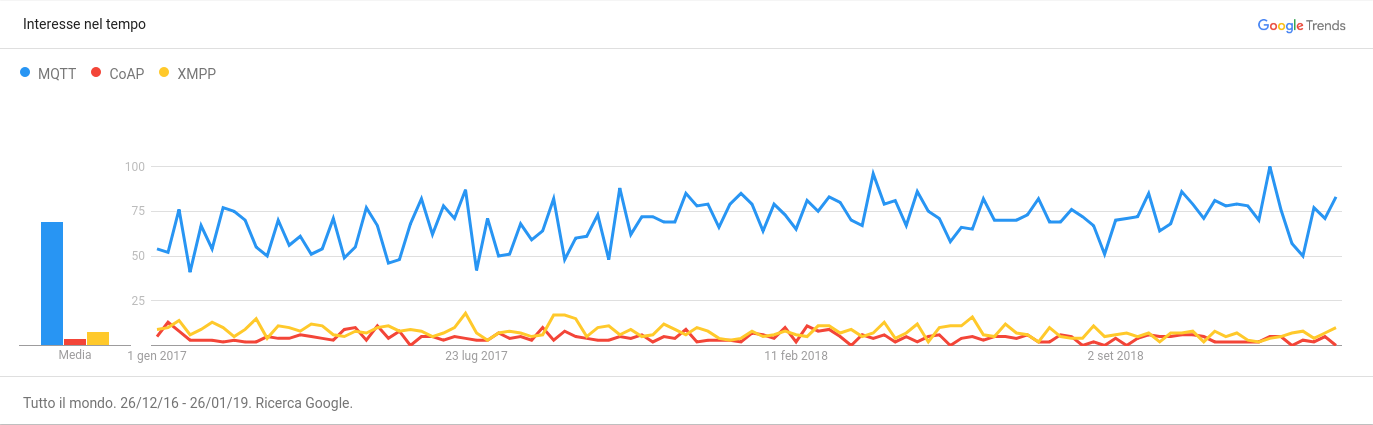
\includegraphics[width=1\textwidth]{trends.png}%
 \caption{Google trends}
 \label{fig:trends}
\end{center}
\end{figure}
Il protocollo che sta avendo maggiormente successo negli ultimi anni, nonostante sia uno dei più recenti, è MQTT: stando agli andamenti di Google Trend (immagine \ref{fig:trends}) l'interesse è almeno 5 volte maggiore di quello del più datato CoAP.

Esistono svariate implementazioni del protocollo MQTT e le numerose librerie open source permettono lo sviluppo di un prototipo in maniera semplice e veloce.

Per questi motivi, ho scelto di implementare una prima versione della piattaforma servendomi di MQTT.

\chapter{Implementazione della piattaforma}
\fancyhead[RO]{\bfseries Implementazione della piattaforma}

La piattaforma deve riuscire a conciliare i bisogni di due attori molto diversi, il publisher e il subscriber.
Il primo, che possiamo identificare nel possessore di un sensore, vuole pubblicare i suoi dati sulla piattaforma in sicurezza e nella maniera più semplice. I subscribers invece, sono tutte le aziende che creano applicazioni utilizzando quei dati, quest'ultimi hanno bisogno di massima integrazione per rendere facile e veloce lo sviluppo e l'adozione del software.
\begin{figure}
\begin{center}
 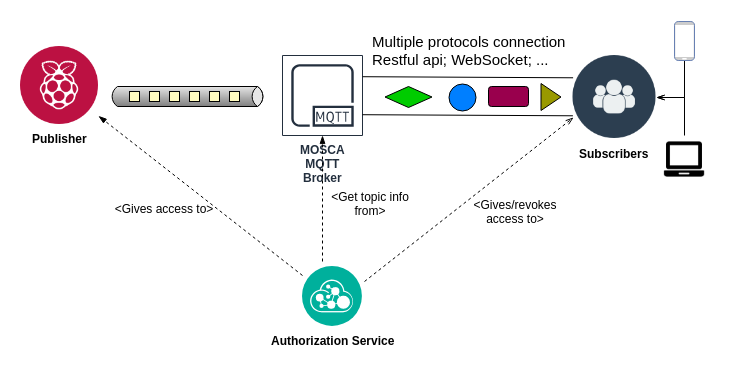
\includegraphics[width=1\textwidth]{architectureSmall.png}%
 \caption{Architecture design}
 \label{fig:architecture}
\end{center}
\end{figure}

Per i motivi sopra citati, si è reso essenziale l'implementazione di un middleware che ho chiamato authorization service (AS). Questa applicazione definisce le modalità di accesso per la pubblicazione e la fruizione dei dati che passano per il broker mqtt. Attraverso questo layer di autenticazione e autorizzazione si può dare massimo controllo dei dati al publisher che ne è il proprietario e che decide a chi dare o revocare l'accesso.

Il broker richiama l'AS per gestire l'autenticazione iniziale del cliente e l'autorizzazione del subscriber durante l'invio dei dati. In questo modo, il publisher, ha una gestione completa dei suoi dati e può decidere a quale subscriber permetterne l'accesso.

La comunicazione con il broker avviene attraverso Transport Layer Security (TLS) che permette una comunicazione sicura dalla sorgente al destinatario. Infine, per evitare che il broker possa leggere il payload del messaggio e quindi per rendere la comunicazione privata tra i due attori del sistema, ho integrato il protocollo PGP.

Il publisher quindi si registra con l'AS e comincia a pubblicare i dati su un topic. Un altro utente, che vuole diventare subscriber di quel topic, invia una richiesta al publisher per usufruire di quei dati. A questo punto il publisher può:
\begin{itemize}
    \item Rifiutare la richiesta e quindi non permettere all'utente di diventare subscriber dei suoi dai.
    \item Accettare la richiesta e aggiungere la chiave pubblica del richiedente nella catena di chiavi PGP
\end{itemize}
A questo punto un subscriber può cominciare ad usare il flusso dati provenienti dal topic selezionato.

Per implementare la piattaforma sono stati usati due framework: mosca, un broker mqtt scritto con nodejs; django rest framework, un framework python perfetto per la sua velocità di sviluppo e le tantissime librerie open source utilizzabili. Per quanto riguarda invece i db, ho selezionato Postgresql per memorizzare utenti e gestire l'autorizzazione, mentre Redis per permettere un'archiviazione persistente dei messaggi del publisher.

\newpage
\section{Broker}
Esistono vari broker mqtt, ma non molti permettono una gestione dinamica delle autorizzazioni necessaria per lo sviluppo della piattaforma. La scelta del broker da usare è ricaduta su Mosca MQTT. Mosca è un broker mqtt open source scritto in nodejs, le caratteristiche principali che lo hanno reso adatto per l'implementazione della piattaforma sono le seguenti:
\begin{itemize}
\item ampia possibilità di personalizzazione
\item MQTT 3.1 e 3.1.1 compliant
\item Implementa QoS 0 e QoS 1
\item Può essere usato facilmente all'interno di altre applicazioni nodejs.
\item Permette lo storage di pacchetti offline attraverso l'uso di qualsiasi database
\end{itemize}
\subsection{Installazione e configurazione broker Mosca}
Mosca permette una comunicazione sicura tra client e broker, attraverso protocollo TLS.

Per permettere l'autenticazione, il broker invia le credenziali dell'utente all'AS che verifica le credenziali nel db e risponde al broker permettendo o negando l'accesso.
Per permettere una comunicazione sicura tra AS e broker, quest'ultimo deve inserire nell'header delle richieste un API Key condivisa tra i due sistemi.

Un publisher può pubblicare solo su topic composti dal suo username come prima parte, in questo modo ad esempio un utente con username uguale a \textit{rossi} può pubblicare solo su topic composti da \textit{/rossi/*}.
Se è autorizzato a pubblicare, viene richiamato l'AS per salvare il nuovo topic in modo che sia visibile agli utenti che vogliono usufruire di quei dati.
Per evitare di richiamare troppo spesso l'AS, la prima risposta del server è salvata in Redis che funge anche cache del sistema.

Per quanto riguarda il subscriber, le sue richieste verso il broker sono inviate all'AS che ne verifica l'autorizzazione. Un subscriber è autorizzato quando ha inviato una richiesta al publisher e questa è stata accettata.
Anche in questo caso ho usato Redis per sfruttare la cache tra broker e AS.

Il broker definisce 4 eventi:
\begin{itemize}
    \item \emph{authenticate}. Viene richiamato quando un nuovo utente vuole cominciare ad interagire con il broker.
    \item \emph{authorizePublish}. Definisce se un publisher può pubblicare su un topic.
    \item \emph{authorizeSubscribe}. Definisce se un subscriber può \texttt{abbonarsi} ad un topic.
    \item \emph{authorizeForward}. Viene richiamato ogni volta che si deve inviare un messaggio ad un subscriber per verificare se è ancora autorizzato a riceverlo.
\end{itemize}

Un publisher può revocare l'autorizzazione ad un subscriber richiamando l'AS; in questo caso il subscriber non riceverà più i nuovi pacchetti.

\newpage
\section{Authorization Service}
L'authorization service è una RestFul API che permette la gestione degli accessi (autenticazione) e quella dei permessi (autorizzazione) oltre che tutte le azioni per accettare/revocare le richieste dei subscribers.

Per implementare l'AS ho usato Django (jang-goh).
Django è un framework utile per creare applicazioni web, è gratuito e open source ed è scritto in Python. 
Django rest framework permette di espandere le funzionalità di django per creare restful api.
Le caratteristiche principali sono:
\begin{itemize}
    \item \emph{framework modulare}. Ogni progetto di Django comprende varie app o componenti.
    \item Esistono tante componenti gratuite facilmente integrabili nel progetto e utili a sviluppare applicazioni web più velocemente.
    \item Documentazione dell'api \emph{autegenerata.}
\end{itemize}

Il database che ho scelto è Postgresql. Questo database open source è nato nell'Università della California a Berkeley. Le sue caratteristiche principali sono \cite{ionosPostgres}:
\begin{itemize}
    \item Possibilità di domande complesse
    \item Chiavi esterne (foreign keys) per il collegamento di dati da due tabelle
    \item Trigger che vengono attivati automaticamente in ingresso e controllano, confermano, modificano, eliminano o in alternativa inseriscono i dati di riferimento
    \item Visualizzazioni aggiornabili
    \item Concetto di transazione completo
    \item Multiversion Concurrency Control (MVCC) per eseguire in modo efficiente l’accesso simultaneo al database
    \item Supporta JSON
\end{itemize}

Le tabelle che ho definito sono: User, Profile, Topic, Request, API keys. 
Queste tabelle sono descritte in figura \ref{fig:database}
\begin{figure}
\begin{center}
  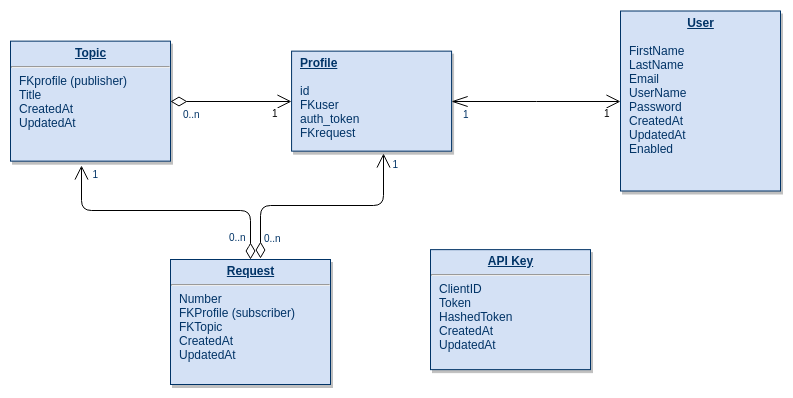
\includegraphics[width=1\textwidth]{database.png}%
  \caption{Database}
  \label{fig:database}
\end{center}
\end{figure}
Di seguito sono descritti tutti gli end-point implementati.

\subsection{Lista delle richieste}
Restituisce la lista delle richieste inviate se viene specificato role=subscriber come parametri nell'url altrimenti quelle ricevute se role=publisher.
\begin{itemize}
\item \textbf{URL} \par
    /request/
\item \textbf{Method} \par
    GET
\item \textbf{URL Params} \par
    [default: role=subscriber] role=[subscriber/publisher]
\item \textbf{Data Params} \par
    None
\item \textbf{Authorization Header} \par
    JWT <token>
\item \textbf{Success Response} \par
    \emph{Code:} 200 \par
    \emph{Content:} [requests list]
\item \textbf{Error Response} \par
    \emph{Code:} 401 UNAUTHORIZED \par
    \emph{Content:} \mint{js}|{"error": [msg] }|
    \emph{Code:} 400 BAD REQUEST \par
    \emph{Content:} \mint{js}|{"error": [msg] }|
\end{itemize}

\subsection{Invio richiesta di accesso al dato}
Crea una nuova richiesta. Inviata dal subscriber al publisher per un topic.
\begin{itemize}
\item \textbf{URL} \par
    /request/
\item \textbf{Method} \par
    POST
\item \textbf{URL Params} \par
    None
\item \textbf{Data Params} \par
    topic: <topic title>
\item \textbf{Authorization Header} \par
    JWT <token>
\item \textbf{Success Response} \par
    \emph{Code:} 200 \par
    \emph{Content:} [created request]
\item \textbf{Error Response} \par
    \emph{Code:} 401 UNAUTHORIZED \par
    \emph{Content:} \mint{js}|{"error": [msg] }|
    \emph{Code:} 400 BAD REQUEST \par
    \emph{Content:} \mint{js}|{"error": [msg] }|
\end{itemize}

\subsection{Acetta o rifiuta una richiesta}
Cambia lo stato di una richiesta per accettarla, cancellarla o rifiutarla
\begin{itemize}
\item \textbf{URL} \par
    /request/
\item \textbf{Method} \par
    PATCH
\item \textbf{URL Params} \par
    None
\item \textbf{Data Params} \par
    topic: <topic title> \par
    subscriber: <subscriber username>
\item \textbf{Authorization Header} \par
    JWT <token>
\item \textbf{Success Response} \par
    \emph{Code:} 200 \par
    \emph{Content:} [updated request]
\item \textbf{Error Response} \par
    \emph{Code:} 401 UNAUTHORIZED \par
    \emph{Content:} \mint{js}|{"error": [msg] }|
    \emph{Code:} 400 BAD REQUEST \par
    \emph{Content:} \mint{js}|{"error": [msg] }|
\end{itemize}

\subsection{Check credenziali della piattaforma}
Controlla le credenziali e ritorna un jwt token da usare in ogni 
chiamata successiva per identificare l'utente.
\begin{itemize}
\item \textbf{URL} \par
    /rest-auth/login/
\item \textbf{Method} \par
    POST
\item \textbf{URL Params} \par
    None
\item \textbf{Data Params} \par
    username; password
\item \textbf{Success Response} \par
    \emph{Code:} 200 \par
    \emph{Content:} [jwt token]
\item \textbf{Error Response} \par
    \emph{Code:} 401 UNAUTHORIZED \par
    \emph{Content:} \mint{js}|{"error": [msg] }|
    \emph{Code:} 400 BAD REQUEST \par
    \emph{Content:} \mint{js}|{"error": [msg] }|
\end{itemize}

\subsection{Lista dei topic}
Restituisce una lista di tutti i topic nel sistema.
\begin{itemize}
\item \textbf{URL} \par
    /topic/
\item \textbf{Method} \par
    GET
\item \textbf{URL Params} \par
    None
\item \textbf{Data Params} \par
    None
\item \textbf{Authorization Header} \par
    JWT <token>
\item \textbf{Success Response} \par
    \emph{Code:} 200 \par
    \emph{Content:} [topic list]
\item \textbf{Error Response} \par
    \emph{Code:} 401 UNAUTHORIZED \par
    \emph{Content:} \mint{js}|{"error": [msg] }|
\end{itemize}

\subsection{MQTT Login [Broker end-point]}
Permette l'autenticazione di un utente rispetto al broker mqtt. Questo endpoint viene richiamato dal broker quando l'utente si vuole autenticare.
\begin{itemize}
\item \textbf{URL} \par
    /login/
\item \textbf{Method} \par
    POST
\item \textbf{URL Params} \par
    None
\item \textbf{Data Params}
    username; password
\item \textbf{Success Response} \par
    \emph{Code:} 200 \par
    \emph{Content:} \mint{js}| {"token": [str]} |
\item \textbf{Error Response} \par
    \emph{Code:} 401 UNAUTHORIZED \par
    \emph{Content:} \mint{js}|{"error": [msg] }|
\end{itemize}


\subsection{Creazione di un topic [Broker end-point]}
Permette la creazione di un nuovo topic.
È il broker mqtt ad eseguire l'azione.
\begin{itemize}
\item \textbf{URL} \par
    /topic/
\item \textbf{Method} \par
    POST
\item \textbf{URL Params} \par
    None
\item \textbf{Data Params} \par
    None
\item \textbf{Header} \par
     Api-Token: YOUR\_API\_TOKEN\_HERE \par
     Api-Secret-Key: YOUR\_API\_SECRET\_KEY\_HERE
\item \textbf{Success Response} \par
    \emph{Code:} 200 \par
    \emph{Content:} [topic created]
\item \textbf{Error Response} \par
    \emph{Code:} 401 UNAUTHORIZED \par
    \emph{Content:} \mint{js}|{"error": [msg] }|
\end{itemize}

\subsection{Subscriber Authorization [Broker end-point]}
Check per verificare che un utente possa diventare un subscriber di un topic.
Verifica che lo stato della richiesta sia in Accepted
\begin{itemize}
\item \textbf{URL} \par
    /auth/
\item \textbf{Method} \par
    POST
\item \textbf{URL Params} \par
    None
\item \textbf{Header} \par
     Api-Token: YOUR\_API\_TOKEN\_HERE \par
     Api-Secret-Key: YOUR\_API\_SECRET\_KEY\_HERE
\item \textbf{Data Params} \par
    username: <subscriber username>
    topic: <topic title>
\item \textbf{Success Response} \par
    \emph{Code:} 200
    \emph{Content:} \mint{js}| {accepted request} |
\item \textbf{Error Response} \par
    \emph{Code:} 401 UNAUTHORIZED \par
    \emph{Content:} \mint{js}|{"error": [msg] }|
\end{itemize}

\subsection{Admin}
Per la gestione dell'AS viene usato l'admin panel di djagno.
Il pannello di gestione è accedibile all'url \textit{/admin/}

Oltre alla possibilità di generare/modificare/cancellare un dato nelle tabelle del db, questa applicazione serve per la creazione degli utenti e delle api Key.
\begin{figure}
\begin{center}
  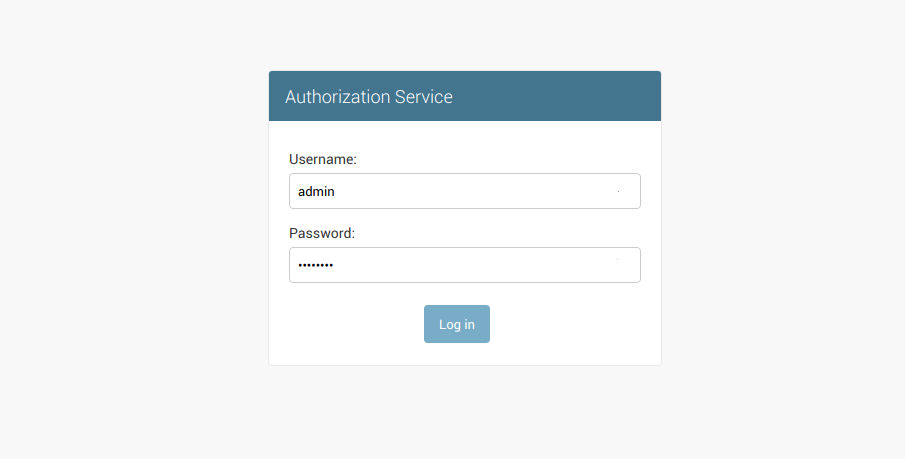
\includegraphics[width=1\textwidth]{LoginAS.png}%
  \caption{Admin login page}
  \label{fig:LoginAS}
\end{center}
\end{figure}
\begin{figure}
\begin{center}
  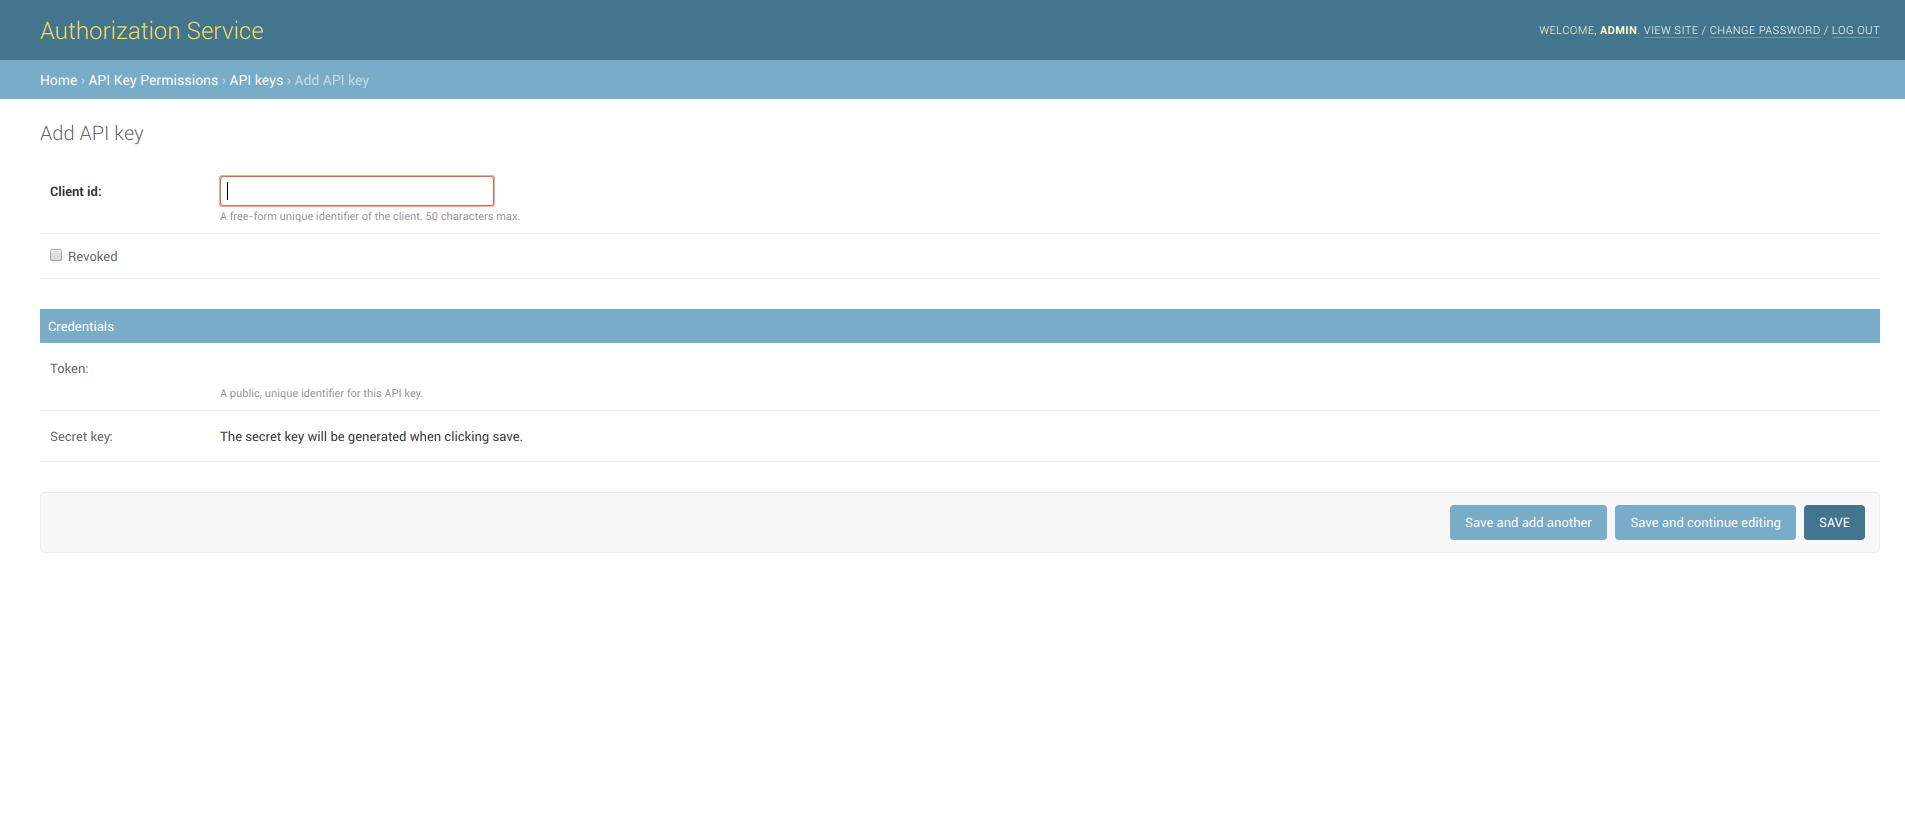
\includegraphics[width=1\textwidth]{images/AddAPIkeyAS.png}%
  \caption{Generate api key}
  \label{fig:AddAPIkeyAS}
\end{center}
\end{figure}
\begin{figure}
\begin{center}
  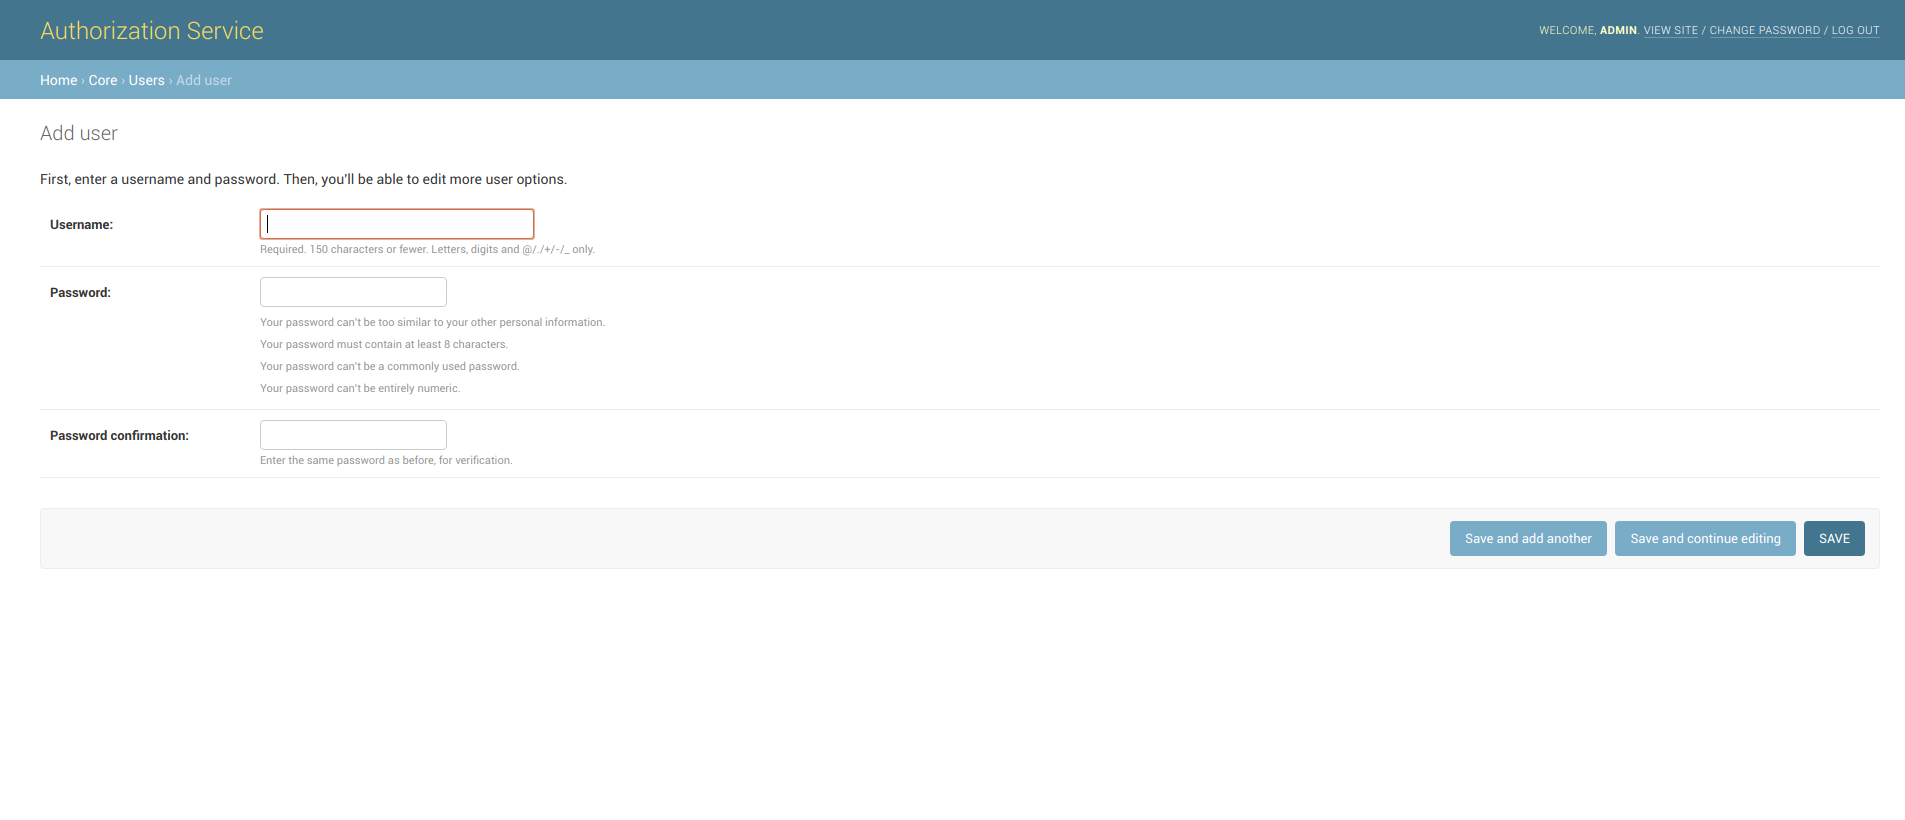
\includegraphics[width=1\textwidth]{images/AddUserAS.png}%
  \caption{Create new user}
  \label{fig:AddUserAS}
\end{center}
\end{figure}

\newpage
\section{Publisher}
Per generare il flusso di dati, ho scelto di usare un raspberry pi e un sensore per misurare il particolato che è una polvere molto fine capace di penetrare facilmente nell'apparato respiratorio.
Riguardo la dimensione delle polveri, è stata fatta una distinzione tra PM10 e PM2.5: PM10 si riferisce alle particelle più piccole di 10µm; PM2.5 sono particelle più piccole di 2.5µm. L'organizzazione Mondiale della Sanità ha fissato i limiti a:
\begin{itemize}
    \item PM10 20 µg/m³ di media l'anno
    \item PM2,5 10 µg/m³ di media l'anno
    \item PM10 50 µg/m³ di media al giorno
    \item PM2,5 25 µg/m³ di media al giorno
\end{itemize}
Nella comunità europea il limite per i PM10 è di 40 µg/m³ l'anno.

\subsection{Sensore Nova SDS011}
Per calcolare il particolato ho usato il sensore Nova SDS011 \ref{fig:sensor}.


\begin{figure}
\begin{center}
  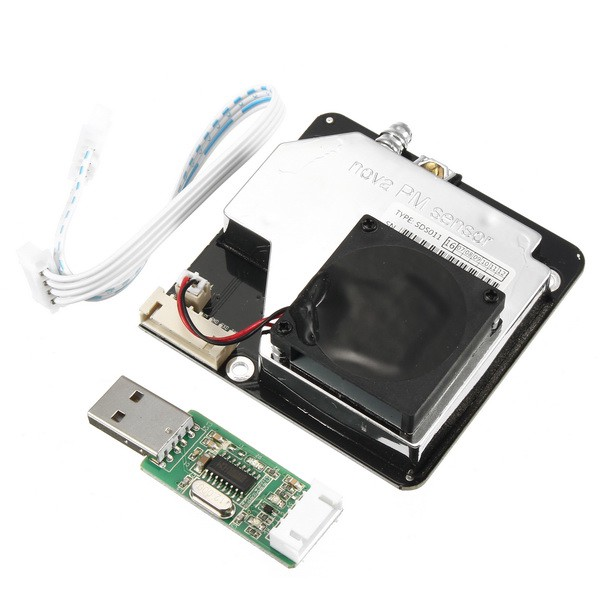
\includegraphics[width=0.6\textwidth]{particulate_sensor.jpg}%
  \caption{SDS011 sensor}
  \label{fig:sensor}
\end{center}
\end{figure}

Il sensore si collega via USB al rasberry pi. Per recuperare i dati del sensore ho usato la libreria javascript \textit{SDS011-Wrapper} \cite{pmSensorGithub}. 



\subsection{Raspberry Pi}
Il raspberry Pi è un single-board computer sviluppato nel Regno Unito dalla Raspberry Pi Foundation. Broadcom BCM2837B0, Cortex-A53 (ARMv8) 64-bit SoC @ 1.4GHz
Il modello che ho usato è un Raspberry Pi 3 model B. Il "system-on-a-chip" è di fabbricazione Broadcom (BCM2837 per Raspberry Pi 3), ed incorpora un Cortex-A53 64-bit SoC @ 1.4GHz e 1 Gigabyte di memoria. Il sistema usa una scheda SD per il boot e per la memoria non volatile.

Il raspberry non ha un sistema operativo preinstallato. Raspbian è l'os "ufficiale", è basato su Debian ed è stato creato appositamente per il raspberry dalla Raspberry Pi Foundation. 

Una volta connesso alla rete e configurato l'ssh \cite{setupraspberry}, ci si può connettere per iniziare l'implementazione del broker. 

\subsection{Implementazione}
Il flusso di creazione di un publisher è mostrato in figura \ref{fig:publisher}
\begin{figure}
\begin{center}
  
\includegraphics[width=1\textwidth]{publisher.png}%
  \caption{Flusso publisher}
  \label{fig:publisher}
\end{center}
\end{figure}

Ho usato la libreria "mqtt" di nodejs per connettere il client al broker mosca. Ogni volta che arriva una lettura dal sensore, il valore di PM10 è pubblicato sul topic selezionato (pseudo codice \ref{lst:publisher}). Poiché il tempo di vita del sensore è stimato in circa 8000 ore, è importante settare una frequenza di lettura idonea.  

\begin{lstlisting}[language=Python, caption={Publisher Pseudocode}, label={lst:publisher}]
let client = new mqtt broker connection
let topic = "username/tesi/pm10"
let sensor = new sds011 connection
sensor.on('measure', (data) => {
  client.publish(topic, data['PM10'])
});
\end{lstlisting}

Il codice completo è presentato in

\newpage
\section{Subscriber}
Un cliente che vuole diventare subscriber di un topic, deve prima richiedere l'accesso al publisher, che può dare o negare l'accesso. 

Il flusso di accesso all'informazione per un subscriber è mostrato in figura \ref{fig:subscriber}
\begin{figure}
\begin{center}
  
\includegraphics[width=1\textwidth]{subscriber.png}%
  \caption{Flusso subscriber}
  \label{fig:subscriber}
\end{center}
\end{figure}

Il subscriber, attraverso l'authorization service (AS), richiede al publisher l'accesso ai dati, che sempre grazie all'AS può in un primo momento concedere e in seguito revocare l'autorizzazione ai topic su cui sta pubblicando lo stream dati.

\newpage
\section{Sicurezza e E2EE}
Come ho detto all'inizio del capitolo, Mosca permette una comunicazione sicura implementando il protocollo TLS. Nonostante questa precauzione però, il messaggio è ancora visibile al server mqtt. 
Crittografia End-To-End (E2EE) vuol dire che il contenuto di un messaggio è visibile solo al mittente e al destinatario, in questo modo si evita che un intermediario, malevolo o no, possa spiare la conversazione o usare i dati di un utente in modo inappropriato.
\subsection{Pretty Good Privacy}
Il protocollo Pretty Good Privacy (PGP) è molto usato per crittografare una comunicazione one-to-one come ad esempio quella tramite mail in modo da essere sicuri che un messaggio sia letto solo dal destinatario. Esistono diverse varianti del protocollo: PGP, OpenPGP, GPG. 

Il protocollo si basa sull'uso di una coppia di chiavi pubblica/privata. La chiave pubblica è usata per crittografare un messaggio che solo con la chiave privata può essere letto.
Criptare e decriptare un messaggio su un client non è un'operazione efficiente \cite{explainPGPEncryption}.
Un'idea generale di come è implementato il protocollo è visibile in figura \ref{fig:pgp}.
\begin{figure}
\begin{center}
  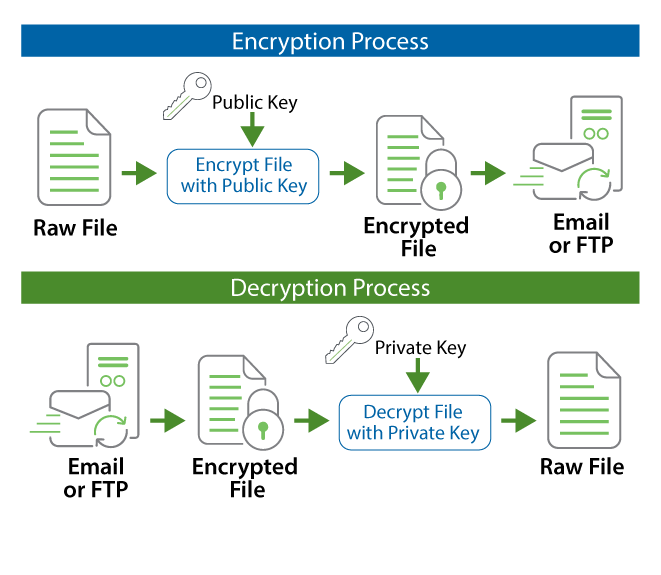
\includegraphics[width=1\textwidth]{images/OpenPGP.png}%
  \caption{PGP System \cite{OpenPGPgoanywhere}}
  \label{fig:pgp}
\end{center}
\end{figure}

PGP permette l'invio di un messaggio criptato a destinatari multipli usando tutte le chiave pubbliche dei destinatari. In questo modo, il mittente, può decidere istantaneamente di escludere un destinatario eliminando la sua chiave pubblica durante la fase di criptazione. 
\subsection{PGP e mqtt}
All'interno della piattaforma ogni cliente, durante la generazione del profilo, carica la propria chiave pubblica.
Nella richiesta per diventare un subscriber viene inserita anche la chiave pubblica dell'utente in modo che quando il publisher accetta la richiesta, questa può essere usata per crittografare il messaggio.
Quando un publisher vuole revocare l'accesso ad un subscriber, può semplicemente eliminare la chiave del subscriber in modo che quest'ultimo non possa più leggere i payloads inviati dal broker.
Il broker MQTT non può leggere i messaggi scambiati all'interno del sistema e si limita alla gestione dei flussi.


\section{Pregi, limiti e prospettive future}
Testo sezione
non è implementato in modo chiaro come avere la lista dei topic
La security è opzionale



%%%%%%%%%%%% CONCLUSIONI   (non numerate come per l'introduzione)
\addcontentsline{toc}{chapter}{conclusioni}
\fancyhead[RO]{\bfseries conclusioni}
\chapter*{Conclusioni}

conclusioni

\newpage 

%%%%%%%%%%%% BIBLIOGRAFIA
\bibliographystyle{abbrvnat}
\bibliography{bibliografia} 
\newpage 

%%%%%%%%%%%% APPENDIX
\appendix
\linespread{1}
\fancyhead[RO]{\bfseries Codice}
\chapter{Codice}
\section{Broker}
\begin{lstlisting}[language=Java, caption={broker.js}, label={lst:broker}]
var mosca = require('mosca')
var redis = require('redis')
const SECURE_KEY = __dirname + './tesi/secure/tls-key.pem';
const SECURE_CERT = __dirname + './tesi/secure/tls-cert.pem';

var backend = {
  type: 'redis',
  redis: redis,
  host: process.env.REDIS_HOST,
  port: process.env.REDIS_PORT,
  db: process.env.REDIS_DB,
  return_buffers: true, // to handle binary payloads
  ttl: {
    subscriptions: 2000
  }
};

var settings = {
  port: 1883,
  backend: backend,
  secure : {
    port: 8443,
    keyPath: SECURE_KEY,
    certPath: SECURE_CERT,
  }
};

var server = new mosca.Server(settings);
server.on('clientConnected', function(client) {
	console.log('client connected', client.id);
});

// fired when a message is received
server.on('published', function(packet, client) {
  console.log('Published', packet.topic, packet.payload);
});

server.on('subscribed', function(packet, client) {
  console.log('Subscribed ', packet.topic, packet.payload);
});

server.on('ready', setup);

// fired when the mqtt server is ready
function setup() {
  console.log('Mosca server is up and running')
}
\end{lstlisting}
\newpage

\section{Topic Listener}
\begin{lstlisting}[language=javascript, caption={topic.js}, label={lst:topic}]
const mqtt = require("mqtt");
const redis = require("redis");
const utils = require("./utils");
const config = require("./config.json");
const topic_url = "topic/";

const redis_client = redis.createClient(
  port = config.redis.port,
  host = config.redis.host
);
redis_client.select(config.redis.db);

 // Number of milliseconds after which a new call
 // to create/delete topics inside the authorization service is done
const API_CALL_INTERVALL = 2000;
 // Number of milliseconds after which a topic is deleted
 // if it doesn't receive data
const TOPIC_EXP = 8000;
// Char used to identify a new topic from one that has already been sent.
// /0 new topic; /1 topic sent
const BIT_NEW = "/0";
const BIT_OLD = "/1";

const client = mqtt.connect(config.broker.host, {
  username: config.broker.username,
  password: config.broker.password
});

client.on("connect", function () {
  // Subscribe to all topic
  // Only staff user can
  client.subscribe('#');
});

client.on("message", function (topic, message) {
  const timestamp = new Date().getTime().toString();
  redis_client.hmget(`topic`, topic, (err, obj) => {
    if (!obj[0]) {
      // Insert a new topic with /0 => to be inserted
      redis_client.hmset(`topic`, topic, timestamp + BIT_NEW);
    } else {
      let bit = obj[0].split('/')[1]
      // Change just the timestamp
      redis_client.hmset(`topic`, topic, timestamp + `/${bit}`);
    }
  });
});

setInterval(
  function () {
    let create_data = [],
      delete_data = [],
      now = new Date().getTime(),
      i,
      topic,
      timestamp,
      bit,
      publisher;
    redis_client.hgetall("topic", function (err, topics) {
      for (topic in topics) {
        timestamp = Number(topics[topic].split("/")[0]);
        bit = Number(topics[topic].split("/")[1]);
        if (now - timestamp > EXP_TIME) {
          // expired
          delete_data.push({
            title: topic
          });
          redis_client.hdel("topic", topic);
        } else if (bit === 0) {
          publisher = topic.split('/')[1];
          // new topics
          create_data.push({
            publisher: publisher,
            title: topic
          });
          redis_client.hmset(
            "topic",
            topic,
            timestamp.toString() + BIT_OLD
          );
        }
      }
      // Call the api to save/delete topics
      const len_create_data = create_data.length;
      const len_delete_data = delete_data.length;
      if (len_create_data > 0) {
        utils.http.post(topic_url, create_data)
        .catch(function (error) {
          // inserisci di nuovo con il char a /0 per riprovare
          timestamp = new Date().getTime();
          for (i = 0; i < create_data.length; i += 1) {
            redis_client.hmset(
              "topic",
              create_data[i]["title"],
              timestamp.toString() + BIT_NEW
            );
          }
        })
      }
      if (len_delete_data > 0) {
        utils.http.delete(topic_url, { data: delete_data })
        .catch(function (error) {
          // inserisci di nuovo con un timestamp scaduto per riprovare
          // now - exp_timestamp > EXP_TIME => true
          let exp_timestamp = Number(now) - EXP_TIME - 1;
          for (i = 0; i < delete_data.length; i += 1) {
            redis_client.hmset(
              "topic",
              delete_data[i]["title"],
              exp_timestamp.toString() + BIT_OLD
            );
          }
        })
      }
    })
  },
  API_CALL_INTERVALL
);
\end{lstlisting}
\newpage

\section{Axios Header API Key}
\begin{footnotesize}
\begin{verbatim}
const http = axios.create({
  baseURL: api_url,
  timeout: 10000,
  headers: {
    'Api-Token': 'c5d87617ceefd2d7b44f2915fd3acbd7',
    'Api-Secret-Key': 'G1V566Zgh5tf'
  }
});
\end{verbatim}
\end{footnotesize}

\newpage
\section{Broker Authentication}
\begin{footnotesize}
\begin{verbatim}
var authenticate = function(client, username, password, callback) {
  const authentication_url = 'mqtt/login/';
  http.post(authentication_url, {
    username: username,
    password: password.toString()
  })
  .then(function (response) {
    // handle success
    const authenticated = response.status === 200;
    if (authenticated) client.user = username;
    callback(null, authenticated);
  })
  .catch(function (error) {
    // handle error
    callback(null, false);
  })
}
\end{verbatim}
\end{footnotesize}

\newpage
\section{Publisher Authentication}
\begin{footnotesize}
\begin{verbatim}
var authorizePublish = function(client, topic, payload, callback) {
  // Authorized only if topic equal to /username/..
  const authorized = client.user == topic.split('/')[1];
  if (authorized) {
    // Try fetching the result from Redis
    redis_client.get(`${client.user}:${topic}`, (err, result) => {
      // If that key exist in Redis store
      if (result === 'false') {
          callback(null, false);
      } else if (result === 'true') {
          callback(null, true);
      } else { // Key does not exist in Redis store
        // Create a new topic associated to the user
        http.post('topic/', {
          title: topic,
          publisher: client.user
        })
        .then(function (response) {
          redis_client.setex(`${client.user}:${topic}`, 3600, response.status < 300);
          callback(null, response.status < 300);
        })
        .catch(function (error) {
          // handle error
          redis_client.setex(`${client.user}:${topic}`, 600, false);
          callback(null, false);
        })
      }
    });
  } else {
    callback(null, false);
  }
}

\end{verbatim}
\end{footnotesize}


\newpage
\section{Subscriber Authorization}
\begin{footnotesize}
\begin{verbatim}

async function canSubscribe(subscriber, topic) {
  const authorization_url = 'mqtt/auth/';
  await http.post(authorization_url, {
    username: subscriber,
    topic: topic
  })
  .then(function (response) {
    // handle success
    console.log(response);
    redis_client.setex(`${subscriber}:subscribe:${topic}`, 3600, response.status < 300);
    return response.status < 300;
  })
  .catch(function (error) {
    // handle error
    redis_client.setex(`${subscriber}:subscribe:${topic}`, 600, false);
    return false;
  })
}

var authorizeForward = function (client, packet, callback) {
  redis_client.get(`${client.user}:subscribe:${packet.topic}`, (err, result) => { 
    if (result === 'false') {
      callback(null, false);
    } else if (result === 'true') {
      callback(null, true);
    } else { // Key does not exist in Redis store
      callback(null, canSubscribe(client, packet.topic))
    }
  })
}
var authorizeSubscribe = function(client, topic, callback) {
  callback(null, canSubscribe(client.user, topic))
}
\end{verbatim}
\end{footnotesize}

\newpage
\section{Publisher}
\begin{footnotesize}
\begin{verbatim}
var mqtt = require('mqtt');
const SDS011Wrapper = require("sds011-wrapper");
const sensor = new SDS011Wrapper("COM5");
Promise
    .all([sensor.setReportingMode('active'), sensor.setWorkingPeriod(10)])
    .then(() => {
        // everything's set
    });
var client = mqtt.connect(`mqtt://${host}`, {
  username: process.env.MQTT_PUBLISHER_USERNAME,
  password: process.env.MQTT_PUBLISHER_PASSWORD
});

client.on('connect', function () {
  sensor.on('measure', (data) => {
    var topic = `/${process.env.MQTT_PUBLISHER_USERNAME}/tesi/pm10`;
    client.publish(topic, data['PM10'])
  });
});
\end{verbatim}
\end{footnotesize}


\newpage
\section{Subscriber}
\begin{footnotesize}
\begin{verbatim}
var mqtt = require('mqtt')
var client = mqtt.connect(`mqtt://${host}`, {
  username: 'subscriber',
  password: 'SgePnQ8fDShnyC3ZdTAy5ZGaW0rSVwVtDVO1QF1kuNs'
});

client.on('connect', function () {
  client.subscribe('/admin/hello')
})

client.on('message', function (topic, message) {
  let context = message.toString();
  console.log(context);
})
\end{verbatim}
\end{footnotesize}

\newpage
\section{Publisher PGP}
\begin{footnotesize}
\begin{verbatim}
const api_url = process.env.API_URL;
const http = axios.create({
  baseURL: api_url,
  timeout: 10000,
  headers: {
    'Authorization': `JWT ${process.env.API_TOKEN}`
  }
});
const privkey = process.env.PRIVATE_KEY;
/**
 * Get the public keys for all the subscribers calling the restful api
 *
 * @param {*} topic
 * @returns array of string
 */
async function getPubKeys(topic) {
  
  // Call api and get subscribers pub keys
  return await http.get(`${topic}/subscribers`)
  .then(function (response) {
    // handle success
    let keys = [];
    console.log(response);
    if (response) {
       for (let i = 0; i < response.length; i++) {
        keys.push(response[i].pubkey)
       }
    }
    return keys
  })
  .catch(function (error) {
    // handle error
    return [];
  })
}


async function encryptWithMultiplePublicKeys(pubkeys, privkey, message) {
  const privKeyObj = (await openpgp.key.readArmored(privkey)).keys[0]

  pubkeys = pubkeys.map(async (key) => {
    return (await openpgp.key.readArmored(key)).keys[0]
  });

  const options = {
      message: openpgp.message.fromText(message),
      publicKeys: pubkeys,           				  // for encryption
      privateKeys: [privKeyObj]                                 // for signing (optional)
  }

  return openpgp.encrypt(options).then(ciphertext => {
      encrypted = ciphertext.data // '-----BEGIN PGP MESSAGE ... END PGP MESSAGE-----'
      return encrypted
  })
};


var client = mqtt.connect('mqtt://localhost', {
  username: process.env.MQTT_USERNAME,
  password: process.env.MQTT_PASSWORD
});

client.on('connect', function () {
  var topic = '/admin/pm10/';
  let pubkeys = getPubKeys(topic);
  setInterval(function() {
    var message = encryptWithMultiplePublicKeys(pubkeys, privkey, '', '100')
    client.publish(topic, message)
    console.log(`Message Sent from ${topic}`);
  }, 20000);
});
\end{verbatim}
\end{footnotesize}


\section{broker.js}
\begin{footnotesize}
\begin{verbatim}
\end{verbatim}
\end{footnotesize}

\end{document}


  
